%%% LaTeX Template: Curriculum Vitae
%%%
%%% Source: http://www.howtotex.com/
%%% Feel free to distribute this template, but please keep the referal to HowToTeX.com.
%%% Date: July 2011

%%% ------------------------------------------------------------
%%% BEGIN PREAMBLE
%%% ------------------------------------------------------------
\documentclass[paper=a4,fontsize=11pt]{scrartcl}	 			% KOMA-article class
							
\usepackage[english]{babel}								% English language/hyphenation
\usepackage[protrusion=true,expansion=true]{microtype}		% Better typography
\usepackage{amsmath,amsfonts,amsthm}					% Math packages
\usepackage[pdftex]{graphicx}								% Enable pdflatex
\usepackage[svgnames]{xcolor}							% Colors by their 'svgnames'
\usepackage{geometry}
	\textheight=700px									% Saving trees ;-) 
\usepackage{url}										% Clickable URL's
\usepackage{wrapfig}									% Wrap text along figures

\frenchspacing									% Better looking spacings after periods
\pagestyle{empty}								% No pagenumbers/headers/footers
\usepackage{bbding}									% Symbols

%%% Custom sectioning (sectsty package)
%%% ------------------------------------------------------------
\usepackage{sectsty}							% Custom sectioning (see below)

\sectionfont{%									% Change font of \section command
	\usefont{OT1}{phv}{b}{n}%					% bch-b-n: CharterBT-Bold font
	\sectionrule{0pt}{0pt}{-5pt}{3pt}
	}

%%% Macros
%%% ------------------------------------------------------------
\newlength{\spacebox}
\settowidth{\spacebox}{8888888888}				% Box to align text
\newcommand{\sepspace}{\vspace*{1em}}			% Vertical space macro

\newcommand{\MyName}[1]{
		\Huge \usefont{OT1}{phv}{b}{n} \hfill #1 		% Name
		\par \normalsize \normalfont}
		
\newcommand{\MySlogan}[1]{
		\large \usefont{OT1}{phv}{m}{n}\hfill \textit{#1} % Slogan (optional)
		\par \normalsize \normalfont}

\newcommand{\NewPart}[1]{\section*{\uppercase{#1}}}

\newcommand{\PersonalEntry}[2]{
		\noindent\hangindent=2em\hangafter=0 		% Indentation
		\parbox{\spacebox}{						% Box to align text
		\textit{#1}}								% Entry name (birth, address, etc.)
		\hspace{1.5em} #2 \par}					% Entry value

\newcommand{\SkillsEntry}[2]{						% Same as \PersonalEntry
		\noindent\hangindent=2em\hangafter=0 		% Indentation
		\parbox{\spacebox}{						% Box to align text
		\textit{#1}}								% Entry name (birth, address, etc.)
		\hspace{1.5em} #2 \par}					% Entry value	
		
\newcommand{\EducationEntry}[4]{
		\noindent \textbf{#1} \hfill 					% Study
		\colorbox{Black}{%
			\parbox{6em}{%
			\hfill\color{White}#2}} \par				% Duration
		\noindent \textit{#3} \par					% School
		\noindent\hangindent=2em\hangafter=0 \small #4 	% Description
		\normalsize \par}

\newcommand{\WorkEntry}[4]{						% Same as \EducationEntry
		\noindent \textbf{#1} \hfill 					% Jobname
		\colorbox{Black}{\color{White}#2} \par		% Duration
		\noindent \textit{#3} \par					% Company
		\noindent\hangindent=2em\hangafter=0 \small #4 	% Description
		\normalsize \par}



%%% ------------------------------------------------------------
%%% BEGIN DOCUMENT
%%% ------------------------------------------------------------
\begin{document}
\begin{wrapfigure}{l}{0.5\textwidth}
	\vspace*{-2em}
		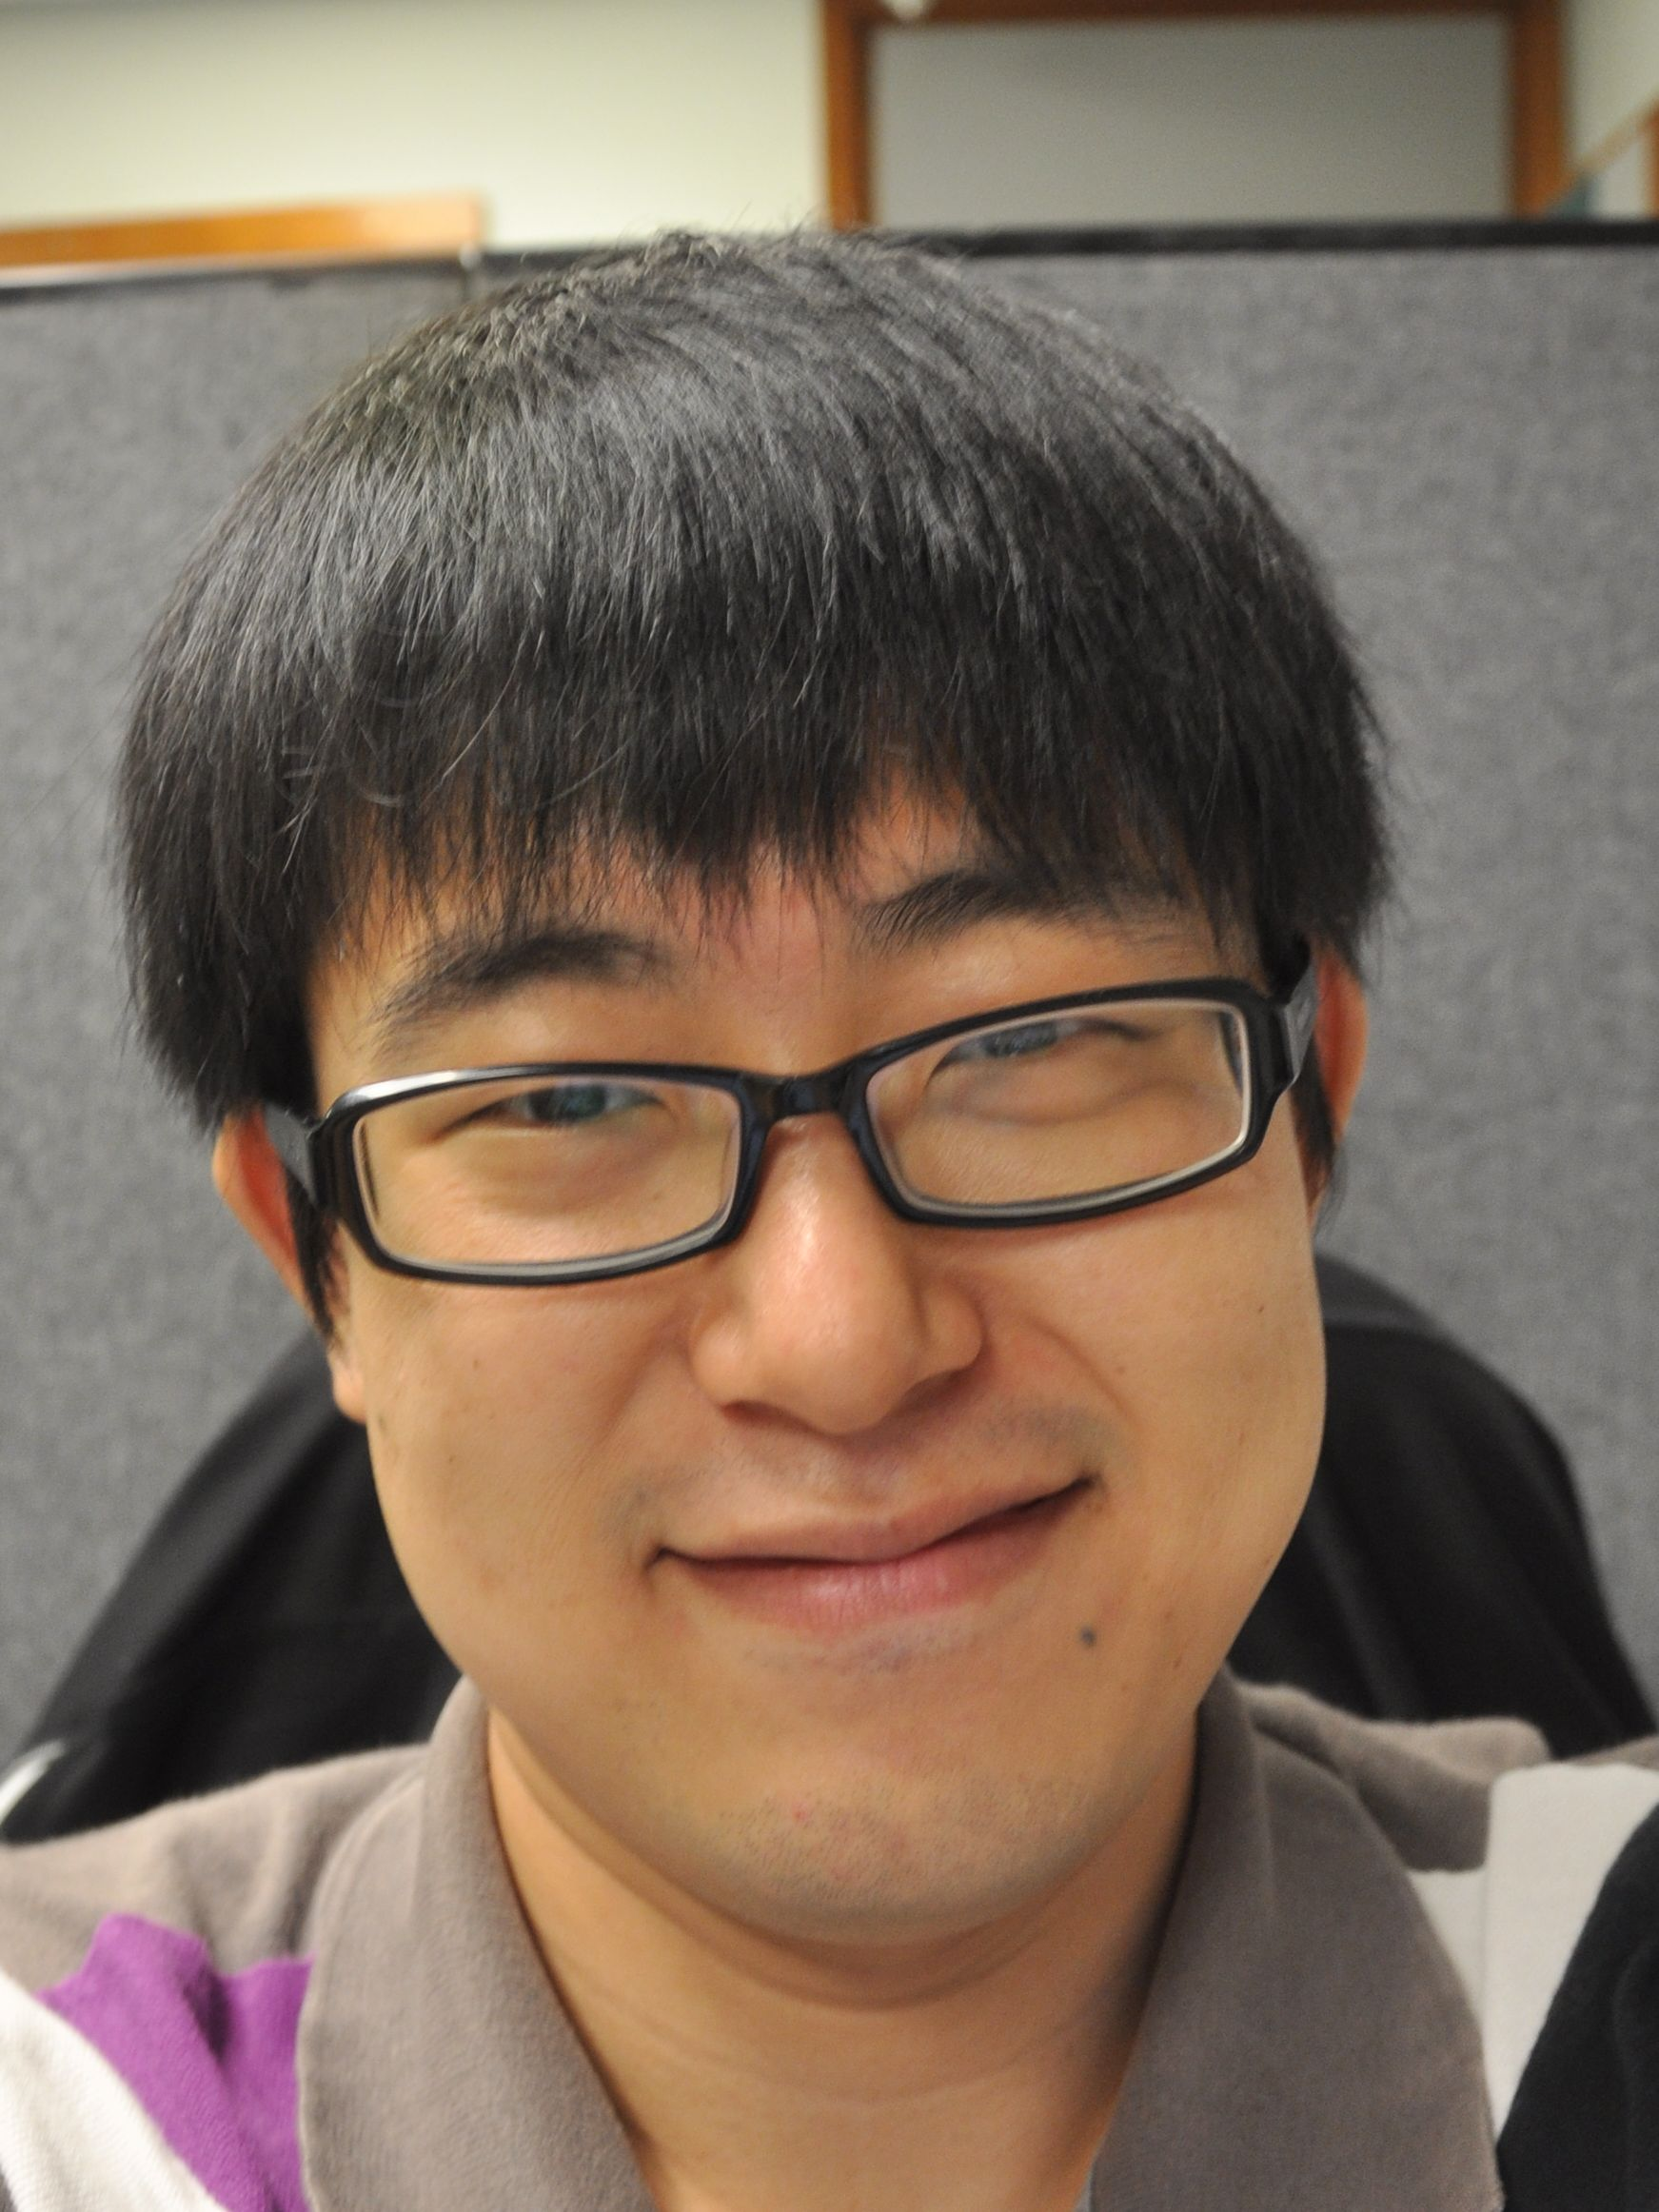
\includegraphics[width=0.15\textwidth]{head}
\end{wrapfigure}

\MyName{Qu Xiaofeng}
\MySlogan{Curriculum Vitae}

\sepspace

%%% Personal details
%%% ------------------------------------------------------------
\NewPart{Personal details}{}

\PersonalEntry{Birth}{March 26, 1982} 
\PersonalEntry{Address}{PQ702, The Hong Kong Polytechnic University, Hong Kong}
\PersonalEntry{Office Tel.}{(852) 2766 7902}
\PersonalEntry{Mail}{\url{csxfqu@comp.polyu.edu.hk}}

%%% Education
%%% ------------------------------------------------------------
\NewPart{Education}{} 

\EducationEntry{Ph.D. Cadidate}{2010-present}{The Hong Kong Polytechnic University}{Majored in Computer Science. Research fields include Computer Vision and Biometrics.}
\sepspace

\EducationEntry{M.E.}{2005-2008}{Shenyang University of Technology, China}{Majored in Detection Technology and Automatic Equipment. Research fields include Machine Vision, Image Processing and Biometrics. Supervised by Prof. Yuan Weiqi. Graduated as Outstanding Graduate with Outstanding Thesis.}
\sepspace

\EducationEntry{B.Eng.}{2001-2005}{Shenyang University of Technology, China}{Majored in Electronic Infomation Engineering. Graduated as Outstading Graduate with Outstanding Project}

%%% Work experience
%%% ------------------------------------------------------------
\NewPart{Employment}{}

\EducationEntry{Research asistant}{2008-2010}{The Hong Kong Polytechnic University, Full-time}{Develop embedded biometric recognition computation platform. Develop ARM, DSP and FPGA based embedded computation platform.}

%%% Skills
%%% ------------------------------------------------------------
\NewPart{Skills}{}

\SkillsEntry{Languages}{Chinese Madarin (mother tongue)}
\SkillsEntry{}{English (fluent)}
\sepspace

\SkillsEntry{Programming}{\textsc{Matlab}, \LaTeX, \textsc{C\slash{}C++}, \textsc{Ruby}}
\sepspace

\SkillsEntry{Engeering}{Electronic device design}
\SkillsEntry{}{Vision system design}
\SkillsEntry{}{DSP, ARM and FPGA development}
\SkillsEntry{}{Protel, Pro/E, WinCE, Linux}

%%% References
%%% ------------------------------------------------------------
\NewPart{References}{}
Available upon request
\end{document}